% !TEX program = pdflatex

\documentclass[12pt]{support/thcolognereport} 

\usepackage{amssymb}

\title{Masterthesis: Optimization of Augmented Reality Applications considering the Depth Information with Googles Project Tango}

\degree{Technical Report}

\author{Steffen Tröster}

\college{Cologne University of Applied Sciences}

\company{inovex GmbH}  

\firstExaminer{Prof. Dr. Hubert Randerath}
\firstExaminerLocation{Technische Hochschule Köln}
\secondExaminer{Prof. Dr. Martin Eisemann}
\secondExaminerLocation{Technische Hochschule Köln}

\degreedate{Cologne, \monthyeardate\today}
	
\begin{document}

\baselineskip=18pt plus1pt

\maketitle 

\setlength{\parskip}{1em}

Project Tango is a new mobile platform by Google’s Advanced Technology and Projects (ATAP) Teams, which brings Motion Tracking, Depth Perception, and Area Learning to smartphones and tablets. This technology can be used to realize real world measurement applications, indoor navigation and virtual reality environments.  With its Motion Tracking technology, Project Tango is also suitable for precise three dimensional augmented reality (AR) applications. The illusion in those applications can be realized by equating the extrinsic and intrinsic camera properties of the real and the virtual camera in a virtual scene. Motion Tracking can then be used to update the virtual camera continuously. But the illusion of the model projection in these AR applications is often disrupted when real objects in the scene are located in front of virtual projections, which are not getting occluded.

The presented thesis is focusing on this augmented reality problem and is comparing three occlusion mechanisms, which can solve the virtual object occlusion with Project Tangos depth perception on mobile hardware and in real time. The applied idea of real world occlusion by the determined depth information was first introduced by \citet{wloka1995resolving}. They are using the z-buffer algorithm and a depth estimation with stereo cameras to prevent a rendering of virtual object parts which are occluded by real object depth information. The presented thesis is indicating three different approaches to fill the z-buffer with depth information captured by the infrared laser sensor, which is integrated in the Project Tango device. It is filled either by the direct sensor data projection, by a TSDF based reconstruction called Chisel by \citet{Klingensmith_2015_7924} or by a self combined and implemented plane based reconstruction. 

Project Tango is not producing a depth map, which could be directly integrated into the z-buffer. It instead is giving a pointcloud with depth information of the current camera perspective. The first naive and already mentioned approach is the projection of the pointcloud to an image plane which then can then be used as z-buffer. The depth sensor is limited to a range of \(50cm\) to \(4m\) and it also has issues capturing depth of complex or reflecting surfaces. Another limitation is the reception rate of only \(5Hz\). Each of these issues are influencing the pointcloud projection due to noise and latency.

\citet{breen1996interactive} are mentioning that the z-buffer based occlusion can also be realized by rendering a primitive based reconstruction as depth map. Therefor the second approach, for solving the mentioned problems, is a plane based reconstruction which got developed during this thesis. It relies on the RANSAC plane estimation from pointclouds by \citet{yang2010plane} and on the plane augmentation and plane range determination method which is used in a SLAM method by \citet{trevor2012planar}. In this approach all incoming points of the depth sensor get collected into an octree with a limited depth for spatial clustering. Than the RANSAC algorithm is applied to all clusters with new points. It either augments existing planes in this cluster or creates new planes with a limit of three planes per cluster. The reach of each plane get calculated and triangulated by the convex hull. 

The second reconstruction and third depth generating approach of this thesis is based on the real time reconstruction field of research. Unlike to offline reconstruction methods like the Poisson reconstruction by \citet{kazhdan2006poisson} or the approach of \citet{hoppe1992surface}, the challenge for real time reconstruction methods is the migration of continues depth information into a single augmenting model. \citet{Klingensmith_2015_7924} has presented a real time reconstruction method based on truncated signed distance fields (TSDF) called Chisel. In this TSDF approach the world is divided into voxel which contain the shortest distance to the next surface. Usually this representation is rendered via raycasting on desktop environments like in KinectFusion by \citet{newcombe2011kinectfusion}. But \citet{Klingensmith_2015_7924} are using the marching cubes method to get a polygon based representation of the surface. They also integrate a spatial hash data structure presented by \citet{niessner2013real} to minimize the footprint of Chisel on mobile devices.

All theses depth map generating approaches producing errors because of noise and limitations in cluster or voxel sizes. Also the plane based reconstruction is producing gaps between planes, which lead to missing depth information in the depth map. Therefor a guided filtering approach by \citet{he2010guided} is applied to the depth map. This filter can interpolate the depth according to the edges of the current color image frame captured by the Project Tango device. 

During this thesis, all these approaches where implemented or ported to the Project Tango development kit as a proof of concept. The final implemented prototype in this thesis is containing all depth generating approaches and also the guided filter which can be combined and manipulated dynamically for an evaluation purpose. The final prototype is shown in figure \ref{fig:filter-demo} and is here just rendering the captured depth map by the TSDF reconstruction and the virtual object, which get occluded by a table top.\\


\begin{figure}[h]
  \centering
	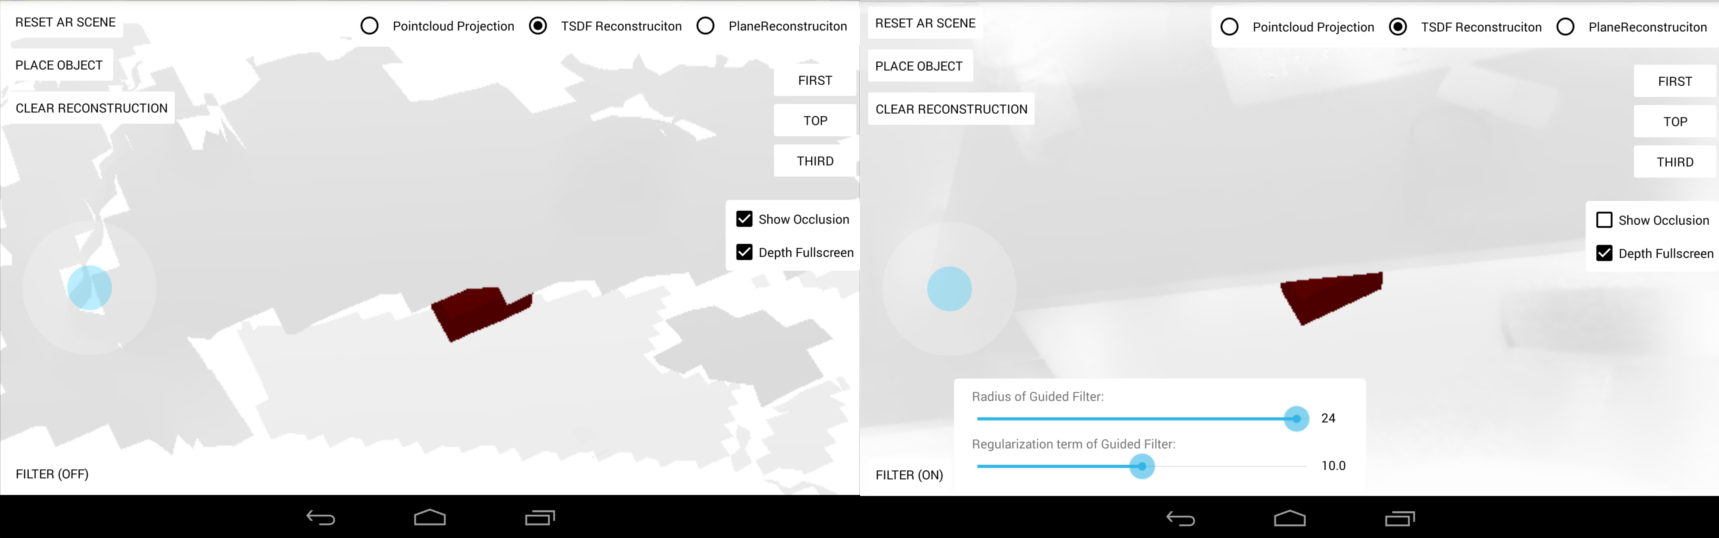
\includegraphics[width=1.0\textwidth]{content/images/implementation/filter-demo.png} 
  \caption{Prototype Screenshot of a Chisel Reconstruction with applied Guided Filter}
  \label{fig:filter-demo}
\end{figure}

\setlength{\parskip}{0em}

\addcontentsline{toc}{chapter}{References}

\bibliography{main}
\bibliographystyle{apalike} 

\end{document}

